\documentclass{ximera}

\usepackage{epsfig}

\graphicspath{
  {./}
  {figures/}
}

\usepackage{epstopdf}
%\usepackage{ulem}
\usepackage[normalem]{ulem}

\epstopdfsetup{outdir=./}

\usepackage{morewrites}
\makeatletter
\newcommand\subfile[1]{%
\renewcommand{\input}[1]{}%
\begingroup\skip@preamble\otherinput{#1}\endgroup\par\vspace{\topsep}
\let\input\otherinput}
\makeatother

\newcommand{\EXER}{}
\newcommand{\includeexercises}{\EXER\directlua{dofile(kpse.find_file("exercises","lua"))}}

\newenvironment{computerExercise}{\begin{exercise}}{\end{exercise}}

%\newcounter{ccounter}
%\setcounter{ccounter}{1}
%\newcommand{\Chapter}[1]{\setcounter{chapter}{\arabic{ccounter}}\chapter{#1}\addtocounter{ccounter}{1}}

%\newcommand{\section}[1]{\section{#1}\setcounter{thm}{0}\setcounter{equation}{0}}

%\renewcommand{\theequation}{\arabic{chapter}.\arabic{section}.\arabic{equation}}
%\renewcommand{\thefigure}{\arabic{chapter}.\arabic{figure}}
%\renewcommand{\thetable}{\arabic{chapter}.\arabic{table}}

%\newcommand{\Sec}[2]{\section{#1}\markright{\arabic{ccounter}.\arabic{section}.#2}\setcounter{equation}{0}\setcounter{thm}{0}\setcounter{figure}{0}}
  
\newcommand{\Sec}[2]{\section{#1}}

\setcounter{secnumdepth}{2}
%\setcounter{secnumdepth}{1} 

%\newcounter{THM}
%\renewcommand{\theTHM}{\arabic{chapter}.\arabic{section}}

\newcommand{\trademark}{{R\!\!\!\!\!\bigcirc}}
%\newtheorem{exercise}{}

\newcommand{\dfield}{{\sf SlopeField}}

\newcommand{\pplane}{{\sf PhasePlane}}

\newcommand{\PPLANE}{{\sf PHASEPLANE}}

% BADBAD: \newcommand{\Bbb}{\bf}. % Package amsfonts Warning: Obsolete command \Bbb; \mathbb should be used instead.

\newcommand{\R}{\mbox{$\mathbb{R}$}}
\let\C\relax
\newcommand{\C}{\mbox{$\mathbb{C}$}}
\newcommand{\Z}{\mbox{$\mathbb{Z}$}}
\newcommand{\N}{\mbox{$\mathbb{N}$}}
\newcommand{\D}{\mbox{{\bf D}}}

\newcommand{\WW}{\mathcal{W}}

\usepackage{amssymb}
%\newcommand{\qed}{\hfill\mbox{\raggedright$\square$} \vspace{1ex}}
%\newcommand{\proof}{\noindent {\bf Proof:} \hspace{0.1in}}

\newcommand{\setmin}{\;\mbox{--}\;}
\newcommand{\Matlab}{{M\small{AT\-LAB}} }
\newcommand{\Matlabp}{{M\small{AT\-LAB}}}
\newcommand{\computer}{\Matlab Instructions}
\renewcommand{\computer}{M\small{ATLAB} Instructions}
\newcommand{\half}{\mbox{$\frac{1}{2}$}}
\newcommand{\compose}{\raisebox{.15ex}{\mbox{{\scriptsize$\circ$}}}}
\newcommand{\AND}{\quad\mbox{and}\quad}
\newcommand{\vect}[2]{\left(\begin{array}{c} #1_1 \\ \vdots \\
 #1_{#2}\end{array}\right)}
\newcommand{\mattwo}[4]{\left(\begin{array}{rr} #1 & #2\\ #3
&#4\end{array}\right)}
\newcommand{\mattwoc}[4]{\left(\begin{array}{cc} #1 & #2\\ #3
&#4\end{array}\right)}
\newcommand{\vectwo}[2]{\left(\begin{array}{r} #1 \\ #2\end{array}\right)}
\newcommand{\vectwoc}[2]{\left(\begin{array}{c} #1 \\ #2\end{array}\right)}

\newcommand{\ignore}[1]{}


\newcommand{\inv}{^{-1}}
\newcommand{\CC}{{\cal C}}
\newcommand{\CCone}{\CC^1}
\newcommand{\Span}{{\rm span}}
\newcommand{\rank}{{\rm rank}}
\newcommand{\trace}{{\rm tr}}
\newcommand{\RE}{{\rm Re}}
\newcommand{\IM}{{\rm Im}}
\newcommand{\nulls}{{\rm null\;space}}

\newcommand{\dps}{\displaystyle}
\newcommand{\arraystart}{\renewcommand{\arraystretch}{1.8}}
\newcommand{\arrayfinish}{\renewcommand{\arraystretch}{1.2}}
\newcommand{\Start}[1]{\vspace{0.08in}\noindent {\bf Section~\ref{#1}}}
\newcommand{\exer}[1]{\noindent {\bf \ref{#1}}}
\newcommand{\ans}{\textbf{Answer:} }
\newcommand{\matthree}[9]{\left(\begin{array}{rrr} #1 & #2 & #3 \\ #4 & #5 & #6
\\ #7 & #8 & #9\end{array}\right)}
\newcommand{\cvectwo}[2]{\left(\begin{array}{c} #1 \\ #2\end{array}\right)}
\newcommand{\cmatthree}[9]{\left(\begin{array}{ccc} #1 & #2 & #3 \\ #4 & #5 &
#6 \\ #7 & #8 & #9\end{array}\right)}
\newcommand{\vecthree}[3]{\left(\begin{array}{r} #1 \\ #2 \\
#3\end{array}\right)}
\newcommand{\cvecthree}[3]{\left(\begin{array}{c} #1 \\ #2 \\
#3\end{array}\right)}
\newcommand{\cmattwo}[4]{\left(\begin{array}{cc} #1 & #2\\ #3
&#4\end{array}\right)}

\newcommand{\Matrix}[1]{\ensuremath{\left(\begin{array}{rrrrrrrrrrrrrrrrrr} #1 \end{array}\right)}}

\newcommand{\Matrixc}[1]{\ensuremath{\left(\begin{array}{cccccccccccc} #1 \end{array}\right)}}



\renewcommand{\labelenumi}{\theenumi}
\newenvironment{enumeratea}%
{\begingroup
 \renewcommand{\theenumi}{\alph{enumi}}
 \renewcommand{\labelenumi}{(\theenumi)}
 \begin{enumerate}}
 {\end{enumerate}
 \endgroup}

\newcounter{help}
\renewcommand{\thehelp}{\thesection.\arabic{equation}}

%\newenvironment{equation*}%
%{\renewcommand\endequation{\eqno (\theequation)* $$}%
%   \begin{equation}}%
%   {\end{equation}\renewcommand\endequation{\eqno \@eqnnum
%$$\global\@ignoretrue}}

%\input{psfig.tex}

\author{Martin Golubitsky and Michael Dellnitz}

%\newenvironment{matlabEquation}%
%{\renewcommand\endequation{\eqno (\theequation*) $$}%
%   \begin{equation}}%
%   {\end{equation}\renewcommand\endequation{\eqno \@eqnnum
% $$\global\@ignoretrue}}

\newcommand{\soln}{\textbf{Solution:} }
\newcommand{\exercap}[1]{\centerline{Figure~\ref{#1}}}
\newcommand{\exercaptwo}[1]{\centerline{Figure~\ref{#1}a\hspace{2.1in}
Figure~\ref{#1}b}}
\newcommand{\exercapthree}[1]{\centerline{Figure~\ref{#1}a\hspace{1.2in}
Figure~\ref{#1}b\hspace{1.2in}Figure~\ref{#1}c}}
\newcommand{\para}{\hspace{0.4in}}

\usepackage{ifluatex}
\ifluatex
\ifcsname displaysolutions\endcsname%
\else
\renewenvironment{solution}{\suppress}{\endsuppress}
\fi
\else
\renewenvironment{solution}{}{}
\fi

\ifcsname answer\endcsname
\renewcommand{\answer}{}
\fi

%\ifxake
%\newenvironment{matlabEquation}{\begin{equation}}{\end{equation}}
%\else
\newenvironment{matlabEquation}%
{\let\oldtheequation\theequation\renewcommand{\theequation}{\oldtheequation*}\begin{equation}}%
  {\end{equation}\let\theequation\oldtheequation}
%\fi

\makeatother

\newcommand{\RED}[1]{{\color{red}{#1}}} 


\title{Gram-Schmidt Orthonormalization Process}

\begin{document}
\begin{abstract}
\end{abstract}
\maketitle

  \label{S:GSO}

\index{Gram-Schmidt orthonormalization}

Suppose that ${\cal W} = \{w_1,\ldots,w_k\}$ is a basis for the subspace
$V\subset\R^n$.  There is a natural process by which the ${\cal W}$ basis
can be transformed into an
orthonormal basis\index{basis!orthonormal}
${\cal V}$ of $V$.  This
process proceeds inductively on the $w_j$; the orthonormal vectors
$v_1,\ldots,v_k$ can be chosen so that
\[
\Span\{v_1,\ldots,v_j\} = \Span\{w_1,\ldots,w_j\}
\]
\index{span}
for each $j\leq k$.  Moreover, the $v_j$ are chosen using the theory of
least squares that we have just discussed.

\subsubsection*{The Case $j=2$}

To gain a feeling for how the induction process works, we verify the case
$j=2$.  Set
\begin{equation}  \label{E:ortho1}
v_1 = \frac{1}{||w_1||}w_1;
\end{equation}
so $v_1$ points in the same direction as $w_1$ and has unit length, that is,
$v_1\cdot v_1=1$.  The normalization is shown in Figure~\ref{F:gram}.

\begin{figure}[htb]
        \centerline{%
        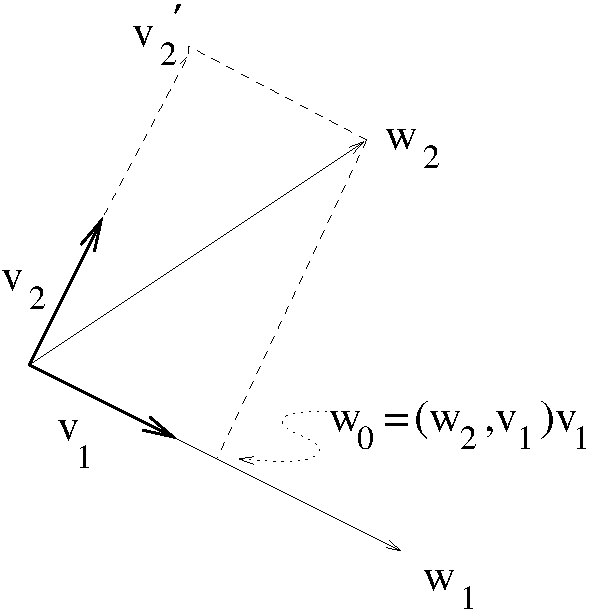
\psfig{file=../figures/gram.eps,width=2.0in}}
        \caption{Planar illustration of Gram-Schmidt orthonormalization.}
        \label{F:gram}
\end{figure}

Next, we find a unit length vector $v'_2$ in the plane spanned by $w_1$ and
$w_2$ that is perpendicular\index{perpendicular}
to $v_1$. Let $w_0$ be the vector on the line
generated by $v_1$ that is nearest to $w_2$.  It follows from
\eqref{E:singleortho} that
\[
w_0 = \frac{w_2\cdot v_1}{||v_1||^2}v_1 = (w_2\cdot v_1) v_1.
\]
The vector $w_0$ is shown on Figure~\ref{F:gram} and, as
Lemma~\ref{L:orthoLSA} states, the vector $v_2'=w_2-w_0$ is perpendicular to
$v_1$. That is,
\begin{equation}  \label{E:ortho2}
v'_2 = w_2 - (w_2\cdot v_1) v_1
\end{equation}
is orthogonal\index{orthogonal} to $v_1$.

Finally, set
\begin{equation}  \label{E:ortho3}
v_2 = \frac{1}{||v'_2||}v'_2
\end{equation}
so that $v_2$ has unit length.  Since $v_2$ and $v'_2$ point in the
same direction, $v_1$ and $v_2$ are orthogonal.  Note also that $v_1$ and
$v_2$ are linear combinations of $w_1$ and $w_2$.  Since $v_1$ and $v_2$ are
orthogonal, they are linearly independent.  It follows that
\[
\Span\{v_1,v_2\} = \Span\{w_1,w_2\}.
\]

In summary: computing $v_1$ and $v_2$ using \eqref{E:ortho1}, \eqref{E:ortho2}
and \eqref{E:ortho3} yields an orthonormal basis for the
plane\index{plane} spanned by $w_1$ and $w_2$.

\subsubsection*{The General Case}

\begin{theorem} (Gram-Schmidt Orthonormalization) \label{T:orthobasis}
Let $w_1,\ldots,w_k$ be a basis for the subspace $W\subset\R^n$.  Define
$v_1$ as in \eqref{E:ortho1} and then define inductively
\begin{align}
  v'_{j+1} & =  w_{j+1} -[(w_{j+1}\cdot v_1)v_1+ \cdots  +(w_{j+1}\cdot v_j)v_j] \label{E:inductiveGS} \\
v_{j+1} & =  \frac{1}{||v'_{j+1}||}v'_{j+1}. \label{eq:gsnormal}
\end{align}
Then $\mathrm{span}\{v_1,\ldots,v_j\}=\mathrm{span}\{w_1,\ldots,w_j\}$ 
and $v_1,\ldots,v_k$ is an orthonormal basis of $W$. 
\end{theorem}\index{Gram-Schmidt orthonormalization}
\index{basis!orthonormal}

\begin{proof}  We assume that we have constructed orthonormal vectors $v_1,\ldots,v_j$
such that
\[
\Span\{v_1,\ldots,v_j\} = \Span\{w_1,\ldots,w_j\}.
\]
Our purpose is to find a unit vector $v_{j+1}$ that is orthogonal to each $v_i$
and that satisfies
\[
\Span\{v_1,\ldots,v_{j+1}\} = \Span\{w_1,\ldots,w_{j+1}\}.
\]
We construct $v_{j+1}$ in two steps.  First we find a vector $v'_{j+1}$
that is orthogonal to each of the $v_i$ using least squares.  Let $w_0$
be the vector in $\Span\{v_1,\ldots,v_j\}$ that is nearest to $w_{j+1}$.
Theorem~\ref{T:nearestvector} tells us how to make this construction.
Let $A$ be the matrix whose columns are $v_1,\ldots,v_j$.  Then
\eqref{E:nearestvector} states that the coordinates of $w_0$ in the $v_i$ basis
is given by $(A^tA)\inv A^tw_{j+1}$. But since the $v_i$'s are orthonormal,
the matrix $A^tA$ is just $I_k$.  Hence
\[
w_0 =  (w_{j+1}\cdot v_1)v_1 + \cdots + (w_{j+1}\cdot v_j)v_j.
\]
Note that $v'_{j+1}=w_{j+1}-w_0$ is the vector defined in \eqref{E:inductiveGS}.
We claim that $v'_{j+1}=w_{j+1}-w_0$ is orthogonal to $v_k$ for $k\leq j$
and hence to every vector in $\Span\{v_1,\ldots,v_j\}$.  Just calculate
\[
v_{j+1}'\cdot v_k = w_{j+1}\cdot v_k - w_0\cdot v_k =
w_{j+1}\cdot v_k -  w_{j+1}\cdot v_k = 0.
\]
Define $v_{j+1}$ as in
\eqref{eq:gsnormal}.  It follows that $v_1,\ldots,v_{j+1}$ are orthonormal and
that each vector is a linear combination of $w_1,\ldots,w_{j+1}$.  \end{proof}


\subsubsection*{An Example of Orthonormalization}

Let $W\subset\R^4$ be the subspace spanned by the vectors
\begin{equation}  \label{eq:gsexam}
w_1=(1,0,-1,0),\quad w_2=(2,-1,0,1),\quad w_3=(0,0,-2,1).
\end{equation}
We find an orthonormal basis for $W$ using Gram-Schmidt orthonormalization.

\begin{description}
\item[Step 1:]   Set
\[
v_1 = \frac{1}{||w_1||}w_1=\frac{1}{\sqrt{2}}(1,0,-1,0).
\]
\item[Step 2:] Following the Gram-Schmidt process, use \eqref{E:inductiveGS} to
define
\begin{align*}
  v'_2 &= w_2-(w_2\cdot v_1)v_1 \\
  &= (2,-1,0,1)-\sqrt{2}\frac{1}{\sqrt{2}}(1,0,-1,0) \\
  &=(1,-1,1,1).
\end{align*}
Normalization using \eqref{eq:gsnormal} yields
\[
v_2 = \frac{1}{||v'_2||}v'_2 = \frac{1}{2}(1,-1,1,1).
\]
\item[Step 3:] Using \eqref{E:inductiveGS} set
\begin{eqnarray*}
v'_3 &=& w_3-(w_3\cdot v_1)v_1-(w_3\cdot v_2)v_2\\
     &=&(0,0,-2,1) - \sqrt{2}\frac{1}{\sqrt{2}}(1,0,-1,0) - \\
         & & \left(-\frac{1}{2}\right)\frac{1}{2}(1,-1,1,1)\\
&=&\frac{1}{4}(-3,-1,-3,5).
\end{eqnarray*}
Normalization using \eqref{eq:gsnormal} yields
\[
v_3 = \frac{1}{||v'_3||}v'_3 = \frac{4}{\sqrt{44}}(-3,-1,-3,5).
\]
\end{description}

Hence we have constructed an orthonormal basis $\{v_1,v_2,v_3\}$ for $W$,
namely
\begin{equation}
\label{eq:gsoresult}
\begin{array}{rcccl}
  v_1 & = & \frac{1}{\sqrt{2}}(1,0,-1,0) \\
      & \approx & (0.7071,0,-0.7071,0)\\
  v_2 & = & \frac{1}{2}(1,-1,1,1) \\
    & = & (0.5,-0.5,0.5,0.5)\\
  v_3 & = & \frac{4}{\sqrt{44}}(-3,-1,-3,5) \\
    & \approx & (-0.4523,-0.1508,-0.4523,0.7538)
\end{array}
\end{equation}




\includeexercises




\end{document}

%%% Local Variables:
%%% mode: latex
%%% TeX-master: "../linearAlgebra"
%%% End:
